\section{Istruzione utilizzo utente responsabile}

La seguente sezione fornirà indicazioni utili per il corretto utilizzo del software nel caso l'utente interessato sia il responsabile.

\subsection{Login}
Il primo passo da effettuare è l'inserimento del proprio codice identificativo e password all'interno dei campi visualizzati nella pagina di login. Dopo aver premuto il pulsante di conferma, si verrà indirizzati alla pagina dedicata alle funzionalità di amministratore. Nel caso le credenziali inserite non risultino corrette, verrà visualizzato un messaggio d'errore e sarà quindi necessario inserire di nuovo i dati.
\begin{figure}[H]
    \centering
    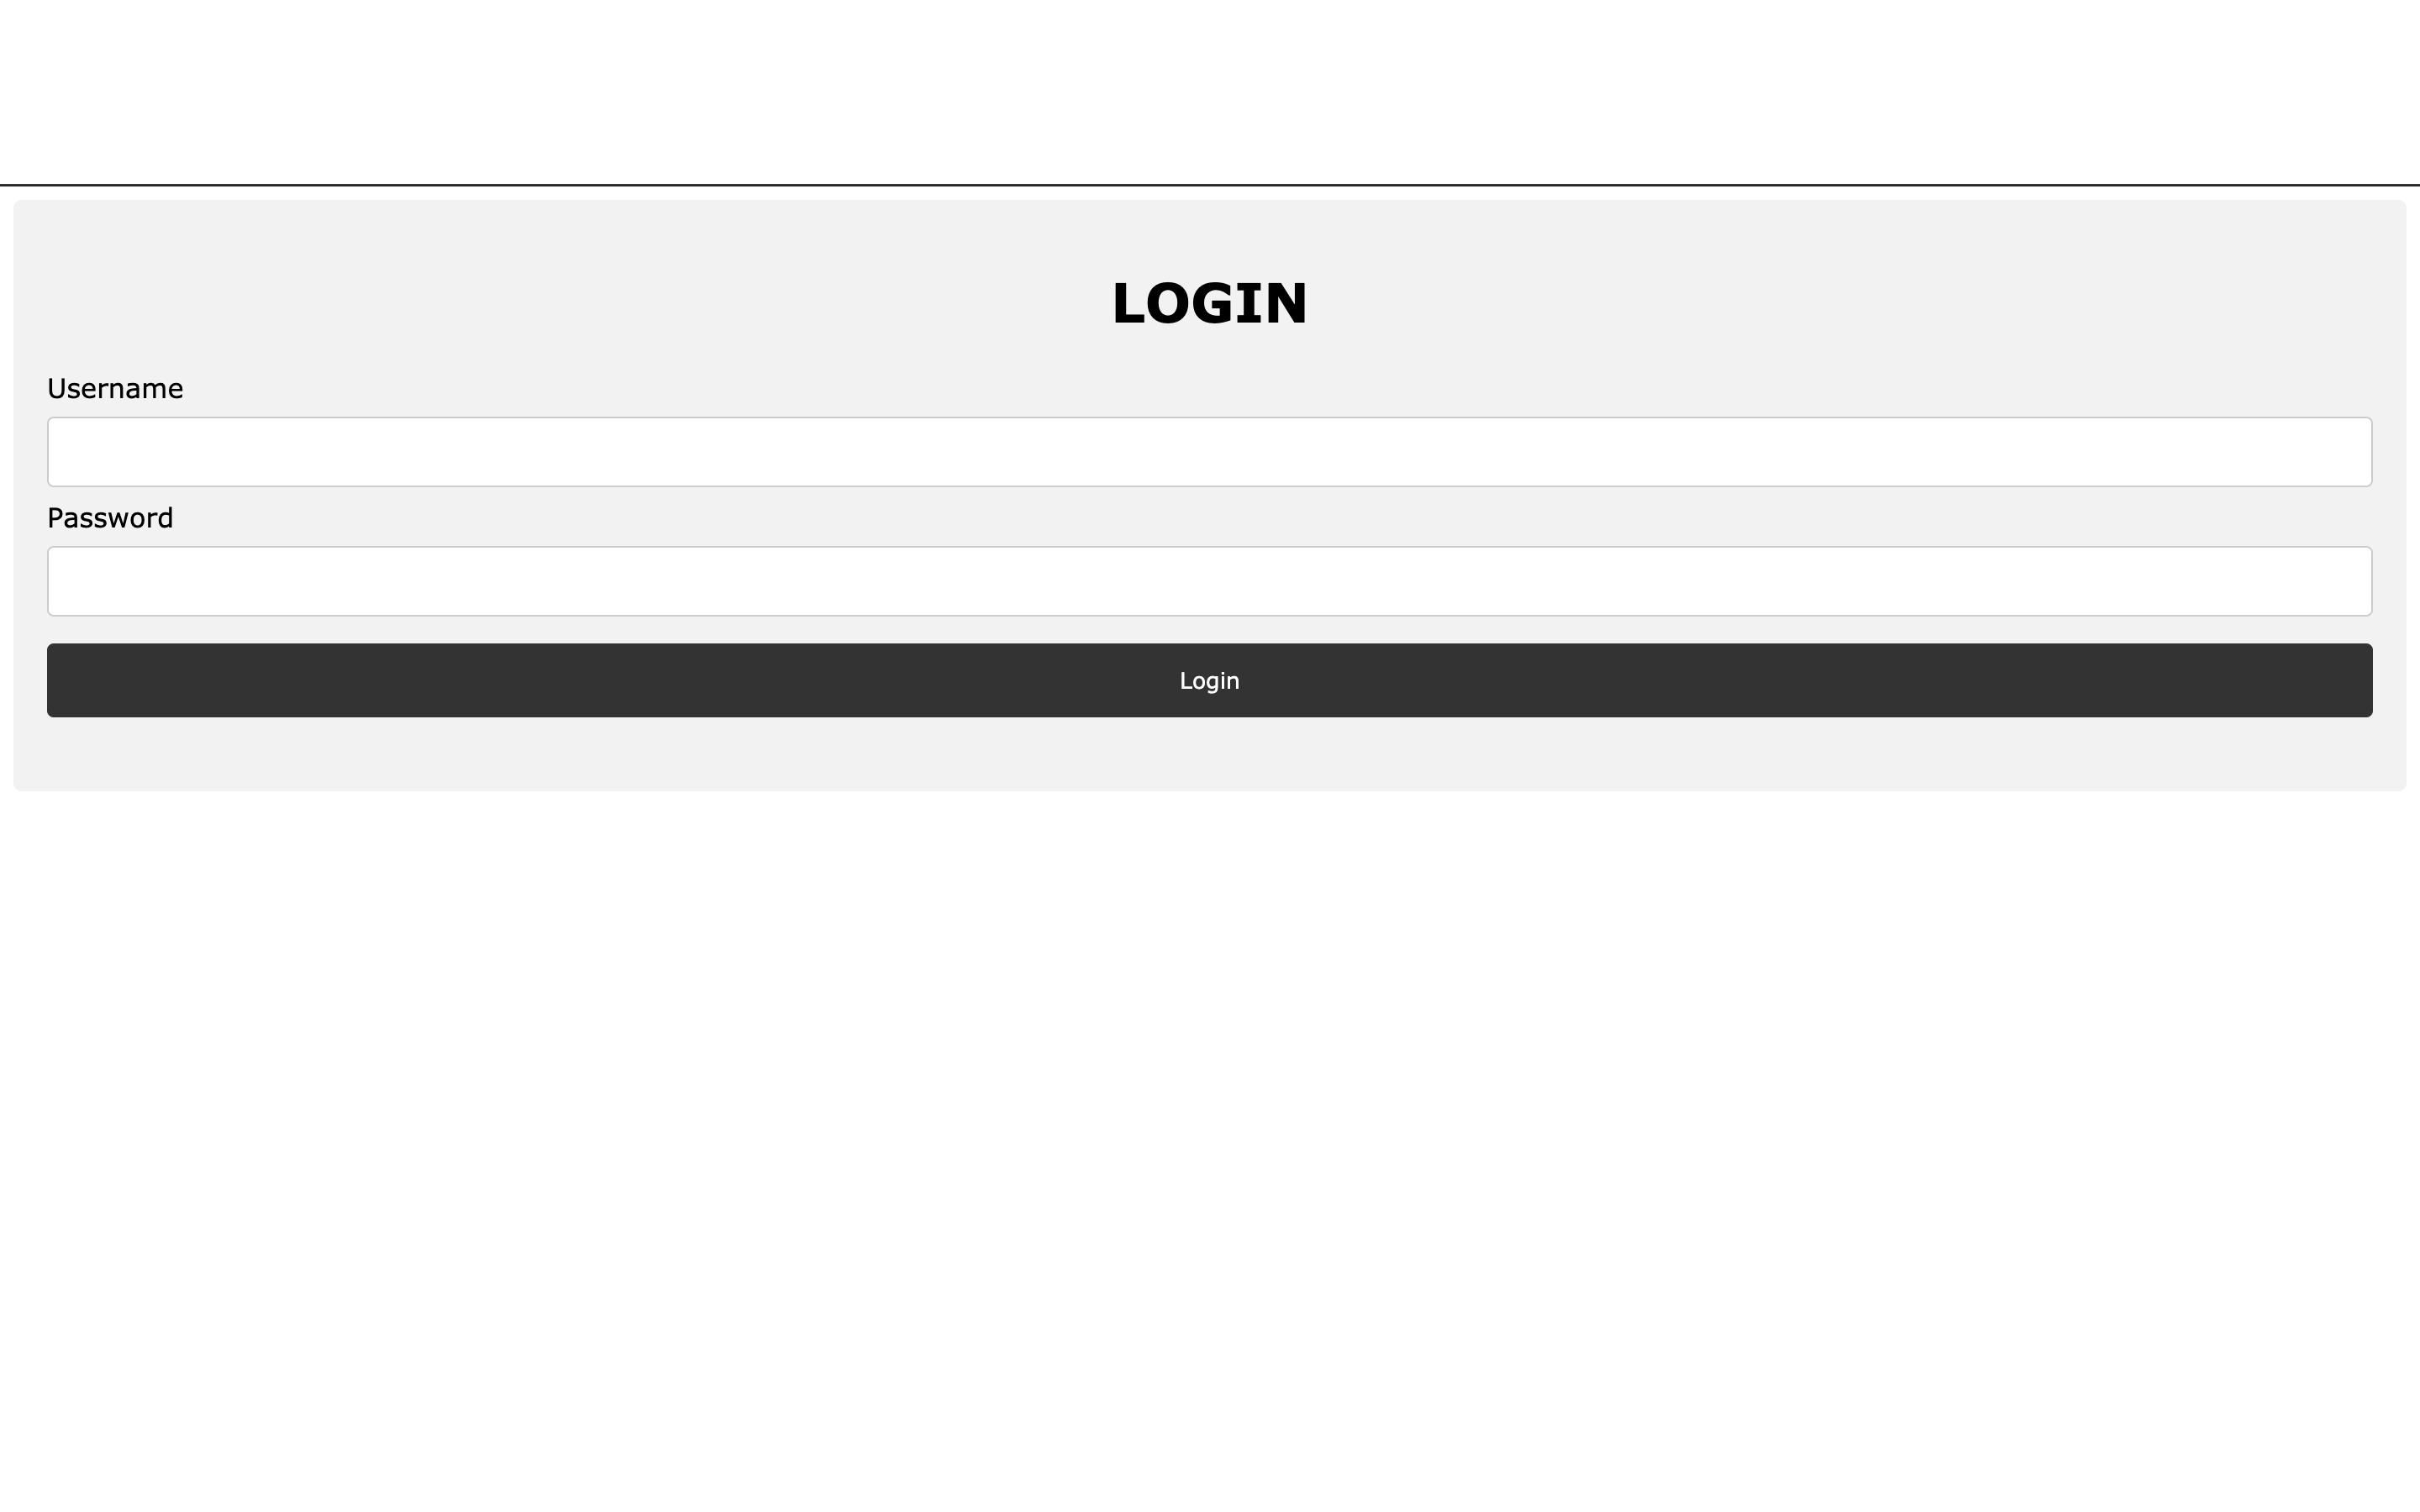
\includegraphics[scale=0.12]{res/images/login.png}
    \caption{Login}
\end{figure}

\subsection{Visualizzazione situazione in real time del magazzino}
\begin{itemize}
    \item Dopo l'autenticazione, tramite il menù selezionare il pulsante "Visualizza mappa";
    \item viene visualizzata la planimetria del magazzino con la relativa legenda e la rappresentazione dei muletti che si spostano;
    
\end{itemize}

\begin{figure}[H]
    \centering
    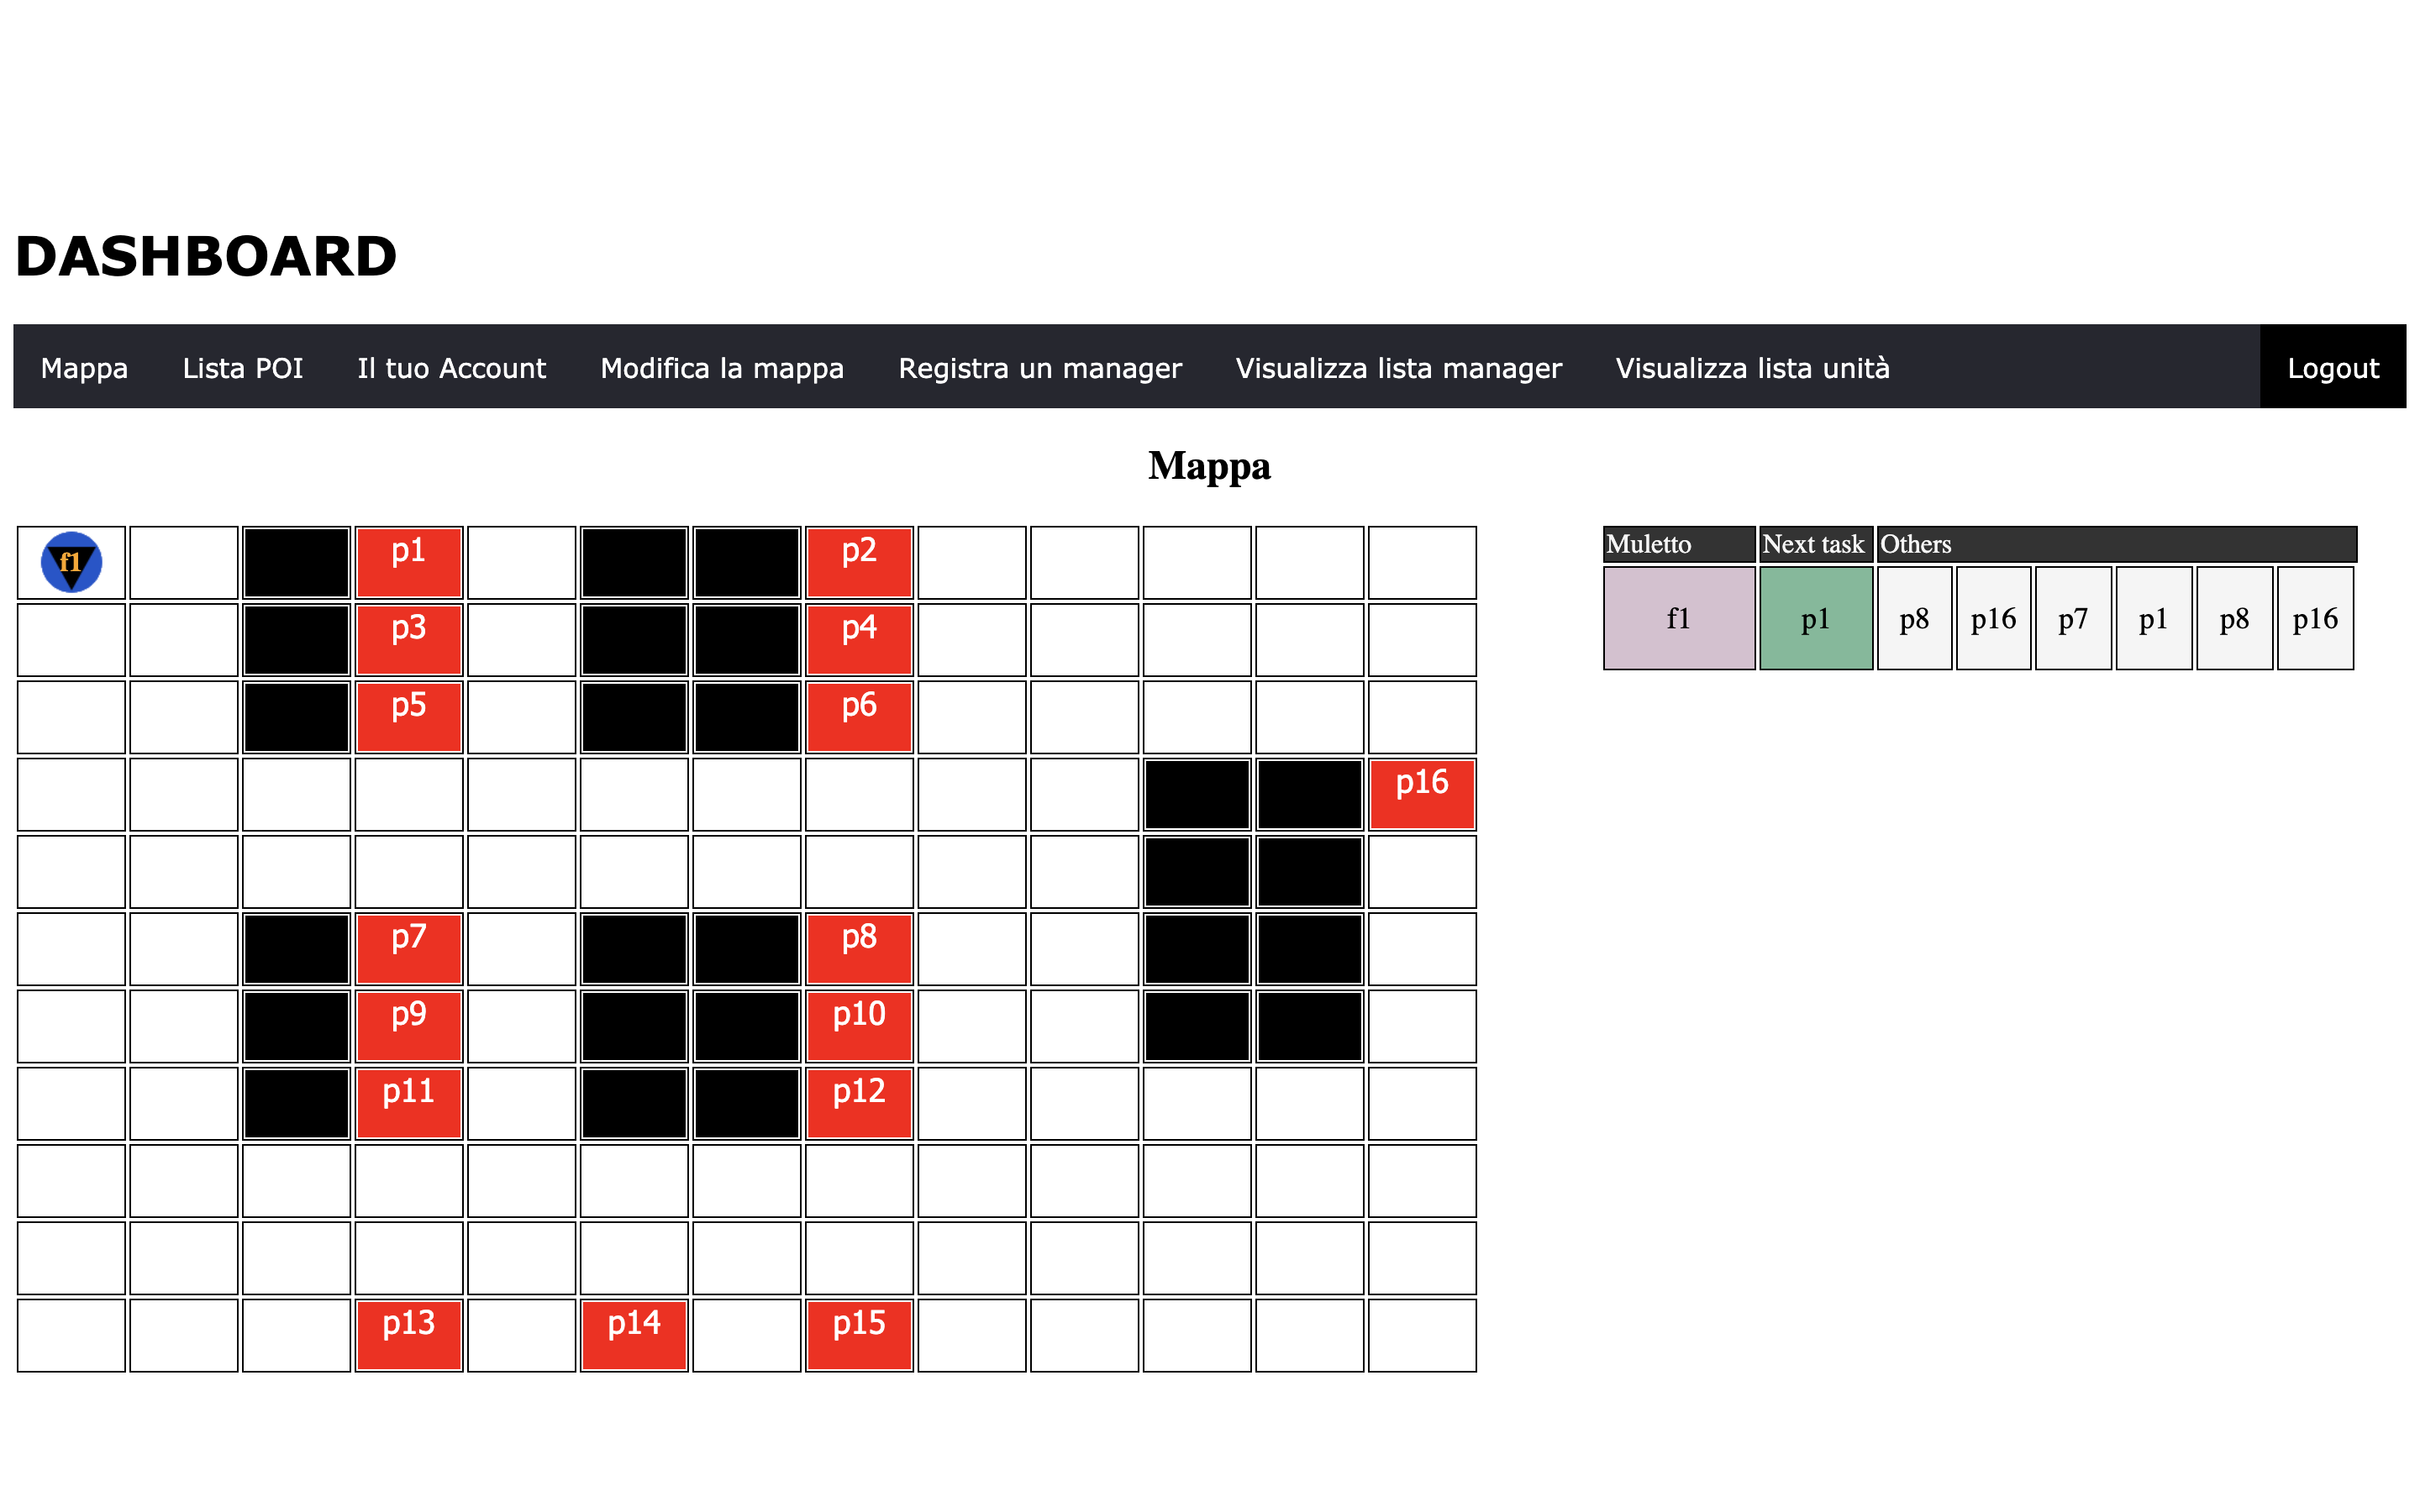
\includegraphics[scale=0.12]{res/images/map_user.png}
    \caption{Schermata guida automatica dell'unità}
\end{figure}

\subsection{Visualizzazione lista completa punti di interesse}
\begin{itemize}
    \item Dopo l'autenticazione, tramite il menù selezionare il pulsante "Visualizza lista POI";
    \item si viene indirizzati alla pagina con l'elenco di tutti i punti di interesse presenti nel magazzino;
    
\end{itemize}

\begin{figure}[H]
    \centering
    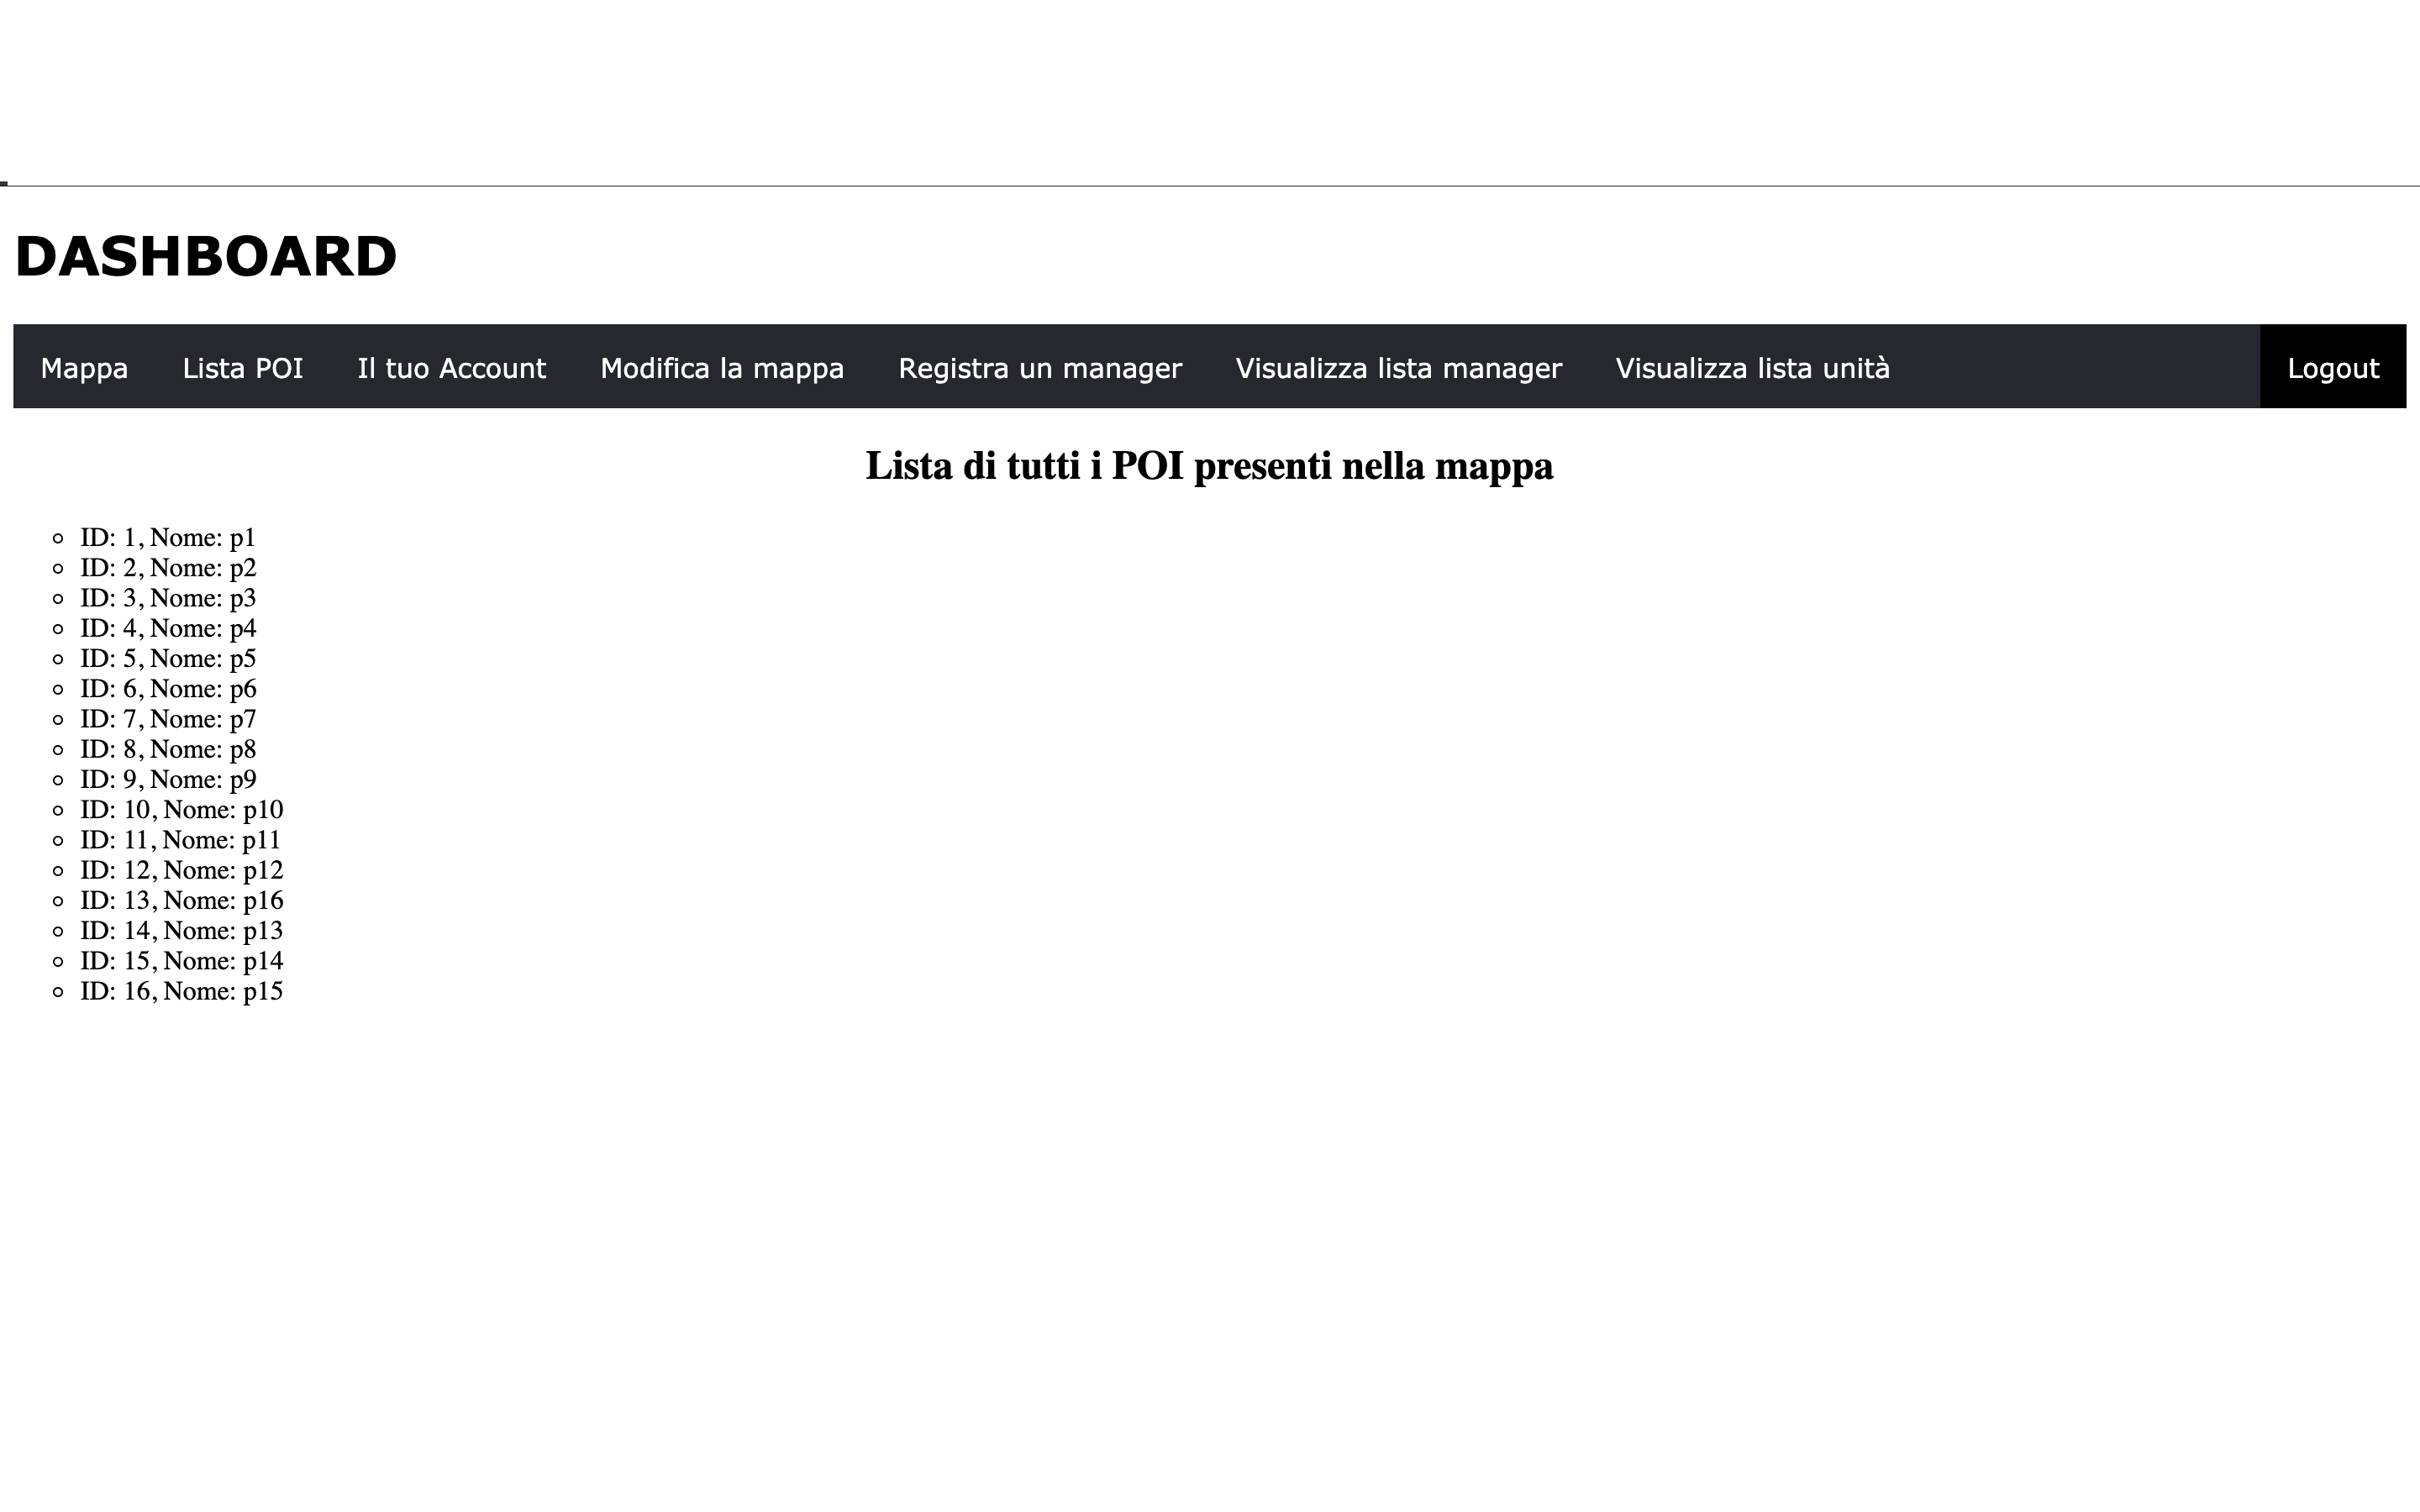
\includegraphics[scale=0.12]{res/images/listpoi_user.png}
    \caption{Schermata guida automatica dell'unità}
\end{figure}

\subsection{Visualizzazione dati del proprio profilo e modifica}
\begin{itemize}
    \item Dopo l'autenticazione, tramite il menù selezionare il pulsante "Visualizza il tuo account";
    \item si viene indirizzati alla pagina con i propri dati utente: nome, cognome, password;
    \item se si desidera modificare alcuni campi, è necessario scrivere nell'apposito form i nuovi dati e premere il pulsante "Conferma";
    
\end{itemize}
\begin{figure}[H]
    \centering
    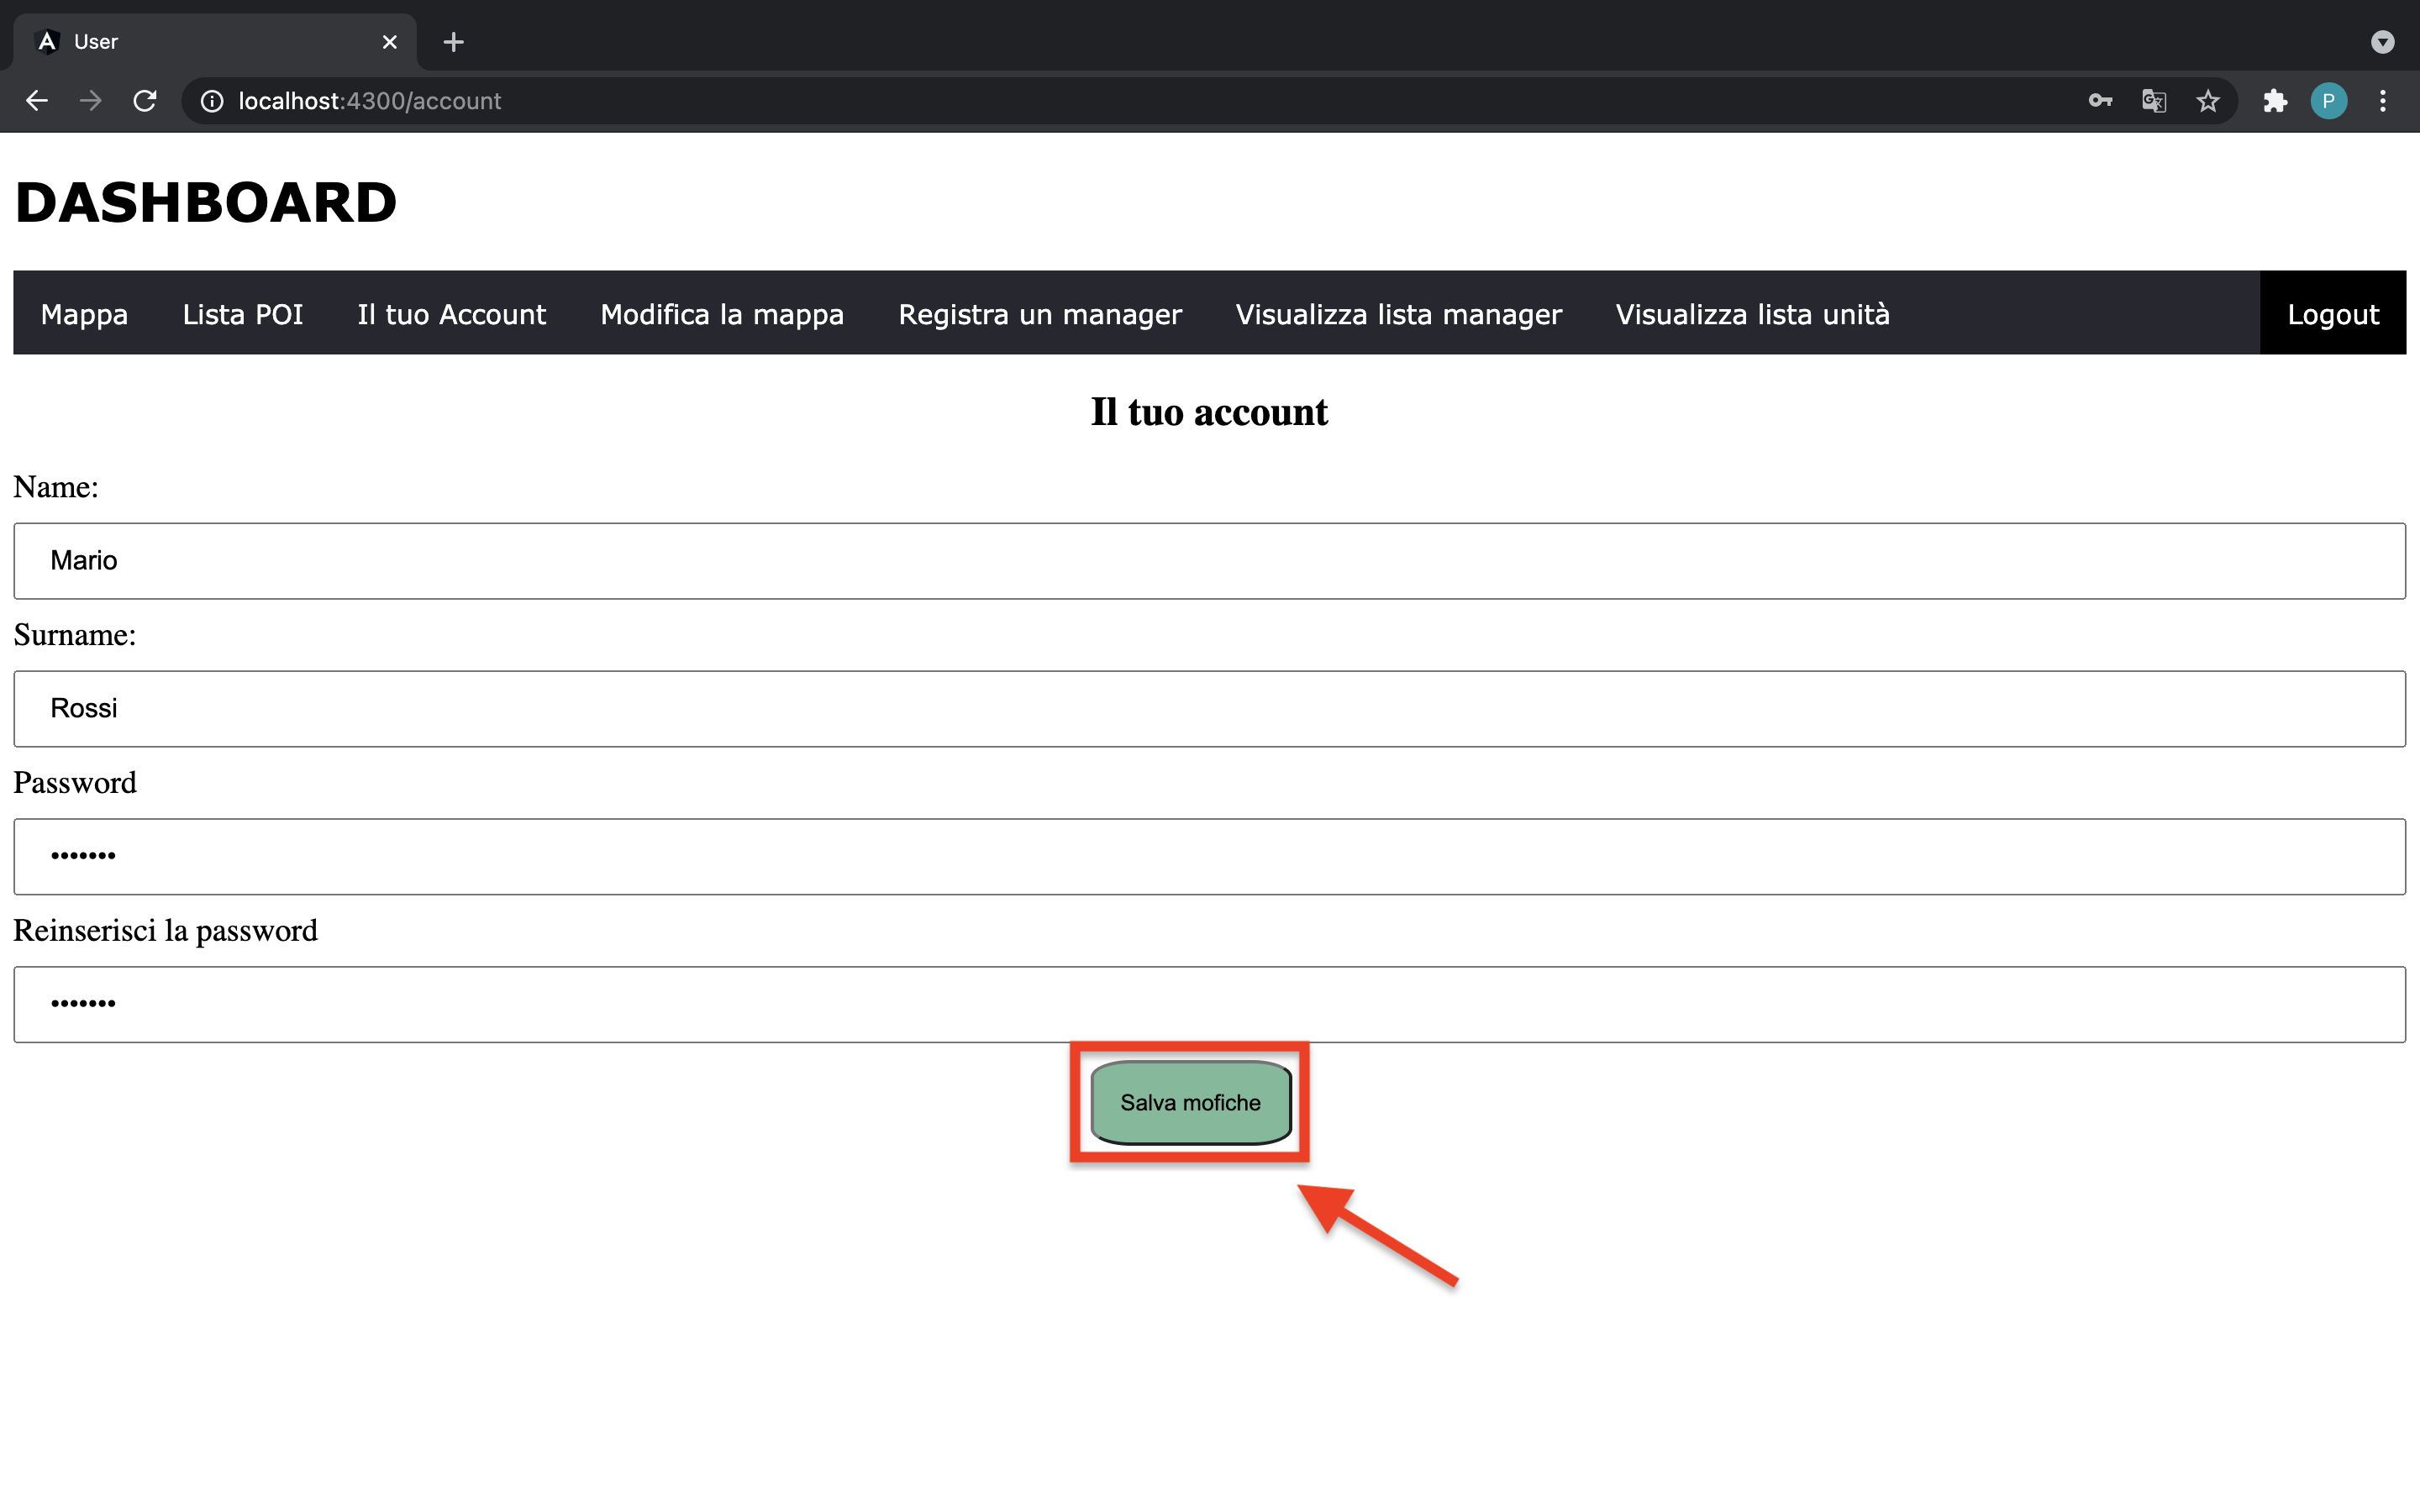
\includegraphics[scale=0.12]{res/images/account_user.png}
    \caption{Schermata guida automatica dell'unità}
\end{figure}

\subsection{Visualizzazione liste di task}
\begin{itemize}
    \item Dopo l'autenticazione, tramite il menù selezionare il pulsante "Visualizza liste di task";
    \item si viene indirizzati alla pagina con due liste: a sinistra le liste assegnate mentre a destra quelle non assegnate.

    
\end{itemize}
\begin{figure}[H]
    \centering
    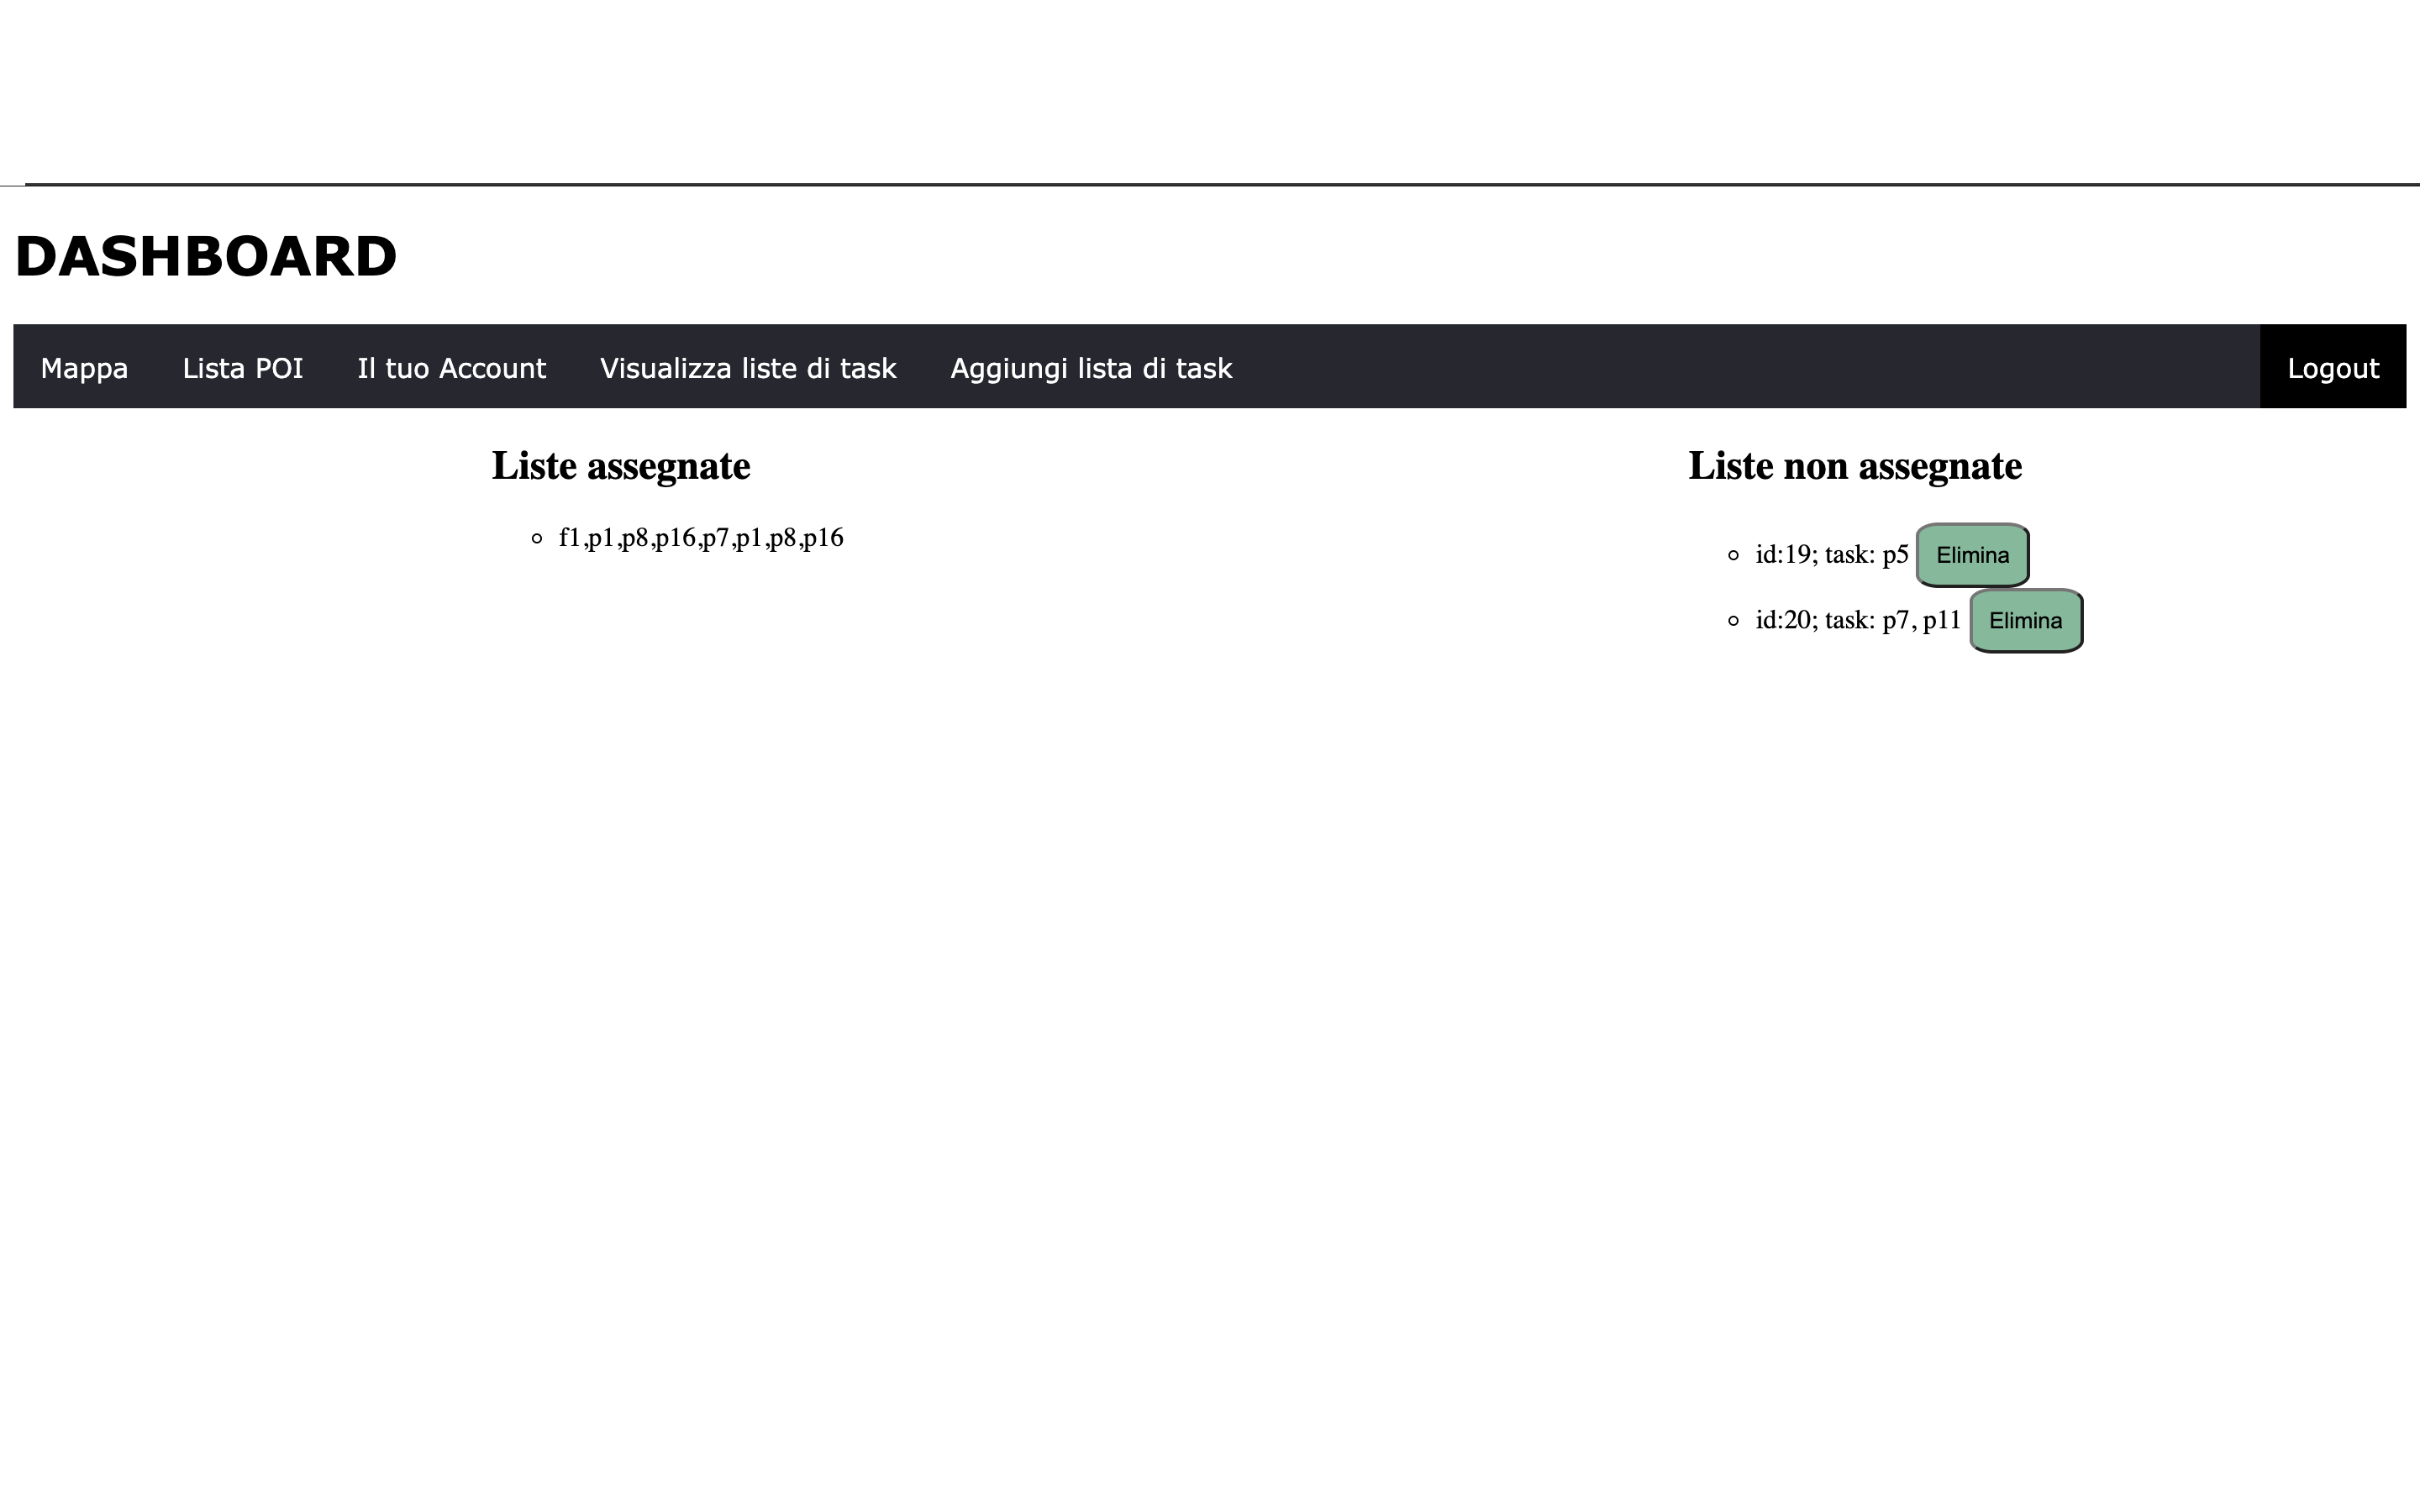
\includegraphics[scale=0.12]{res/images/task_manager.png}
    \caption{Schermata guida automatica dell'unità}
\end{figure}
\subsection{Gestione task}
\begin{itemize}
    \item Dopo l'autenticazione, tramite il menù selezionare il pulsante "Gestisci task";
    \item si viene indirizzati alla pagina con le operazioni per la gestione delle task;
\end{itemize}
\subsubsection{Aggiungere nuova lista di task}
\begin{itemize}
    \item Premere sul pulsante "Aggiungi nuova lista di task"
    \item viene visualizzato un form in cui inserire il POI di interesse e confermare; \\ripetere questo punto per tutte le task che si intendono inserire;
    \item tramite il pulsante "Elimina" di fianco ad ogni task inserita è possibile eliminarla prima di confermare;
    \item una volta aggiunte tutte le task, premere il pulsante "Conferma";
    \item per tornare alla pagina iniziale serve premere sul pulsante "Chiudi".
\end{itemize}

\begin{figure}[H]
    \centering
    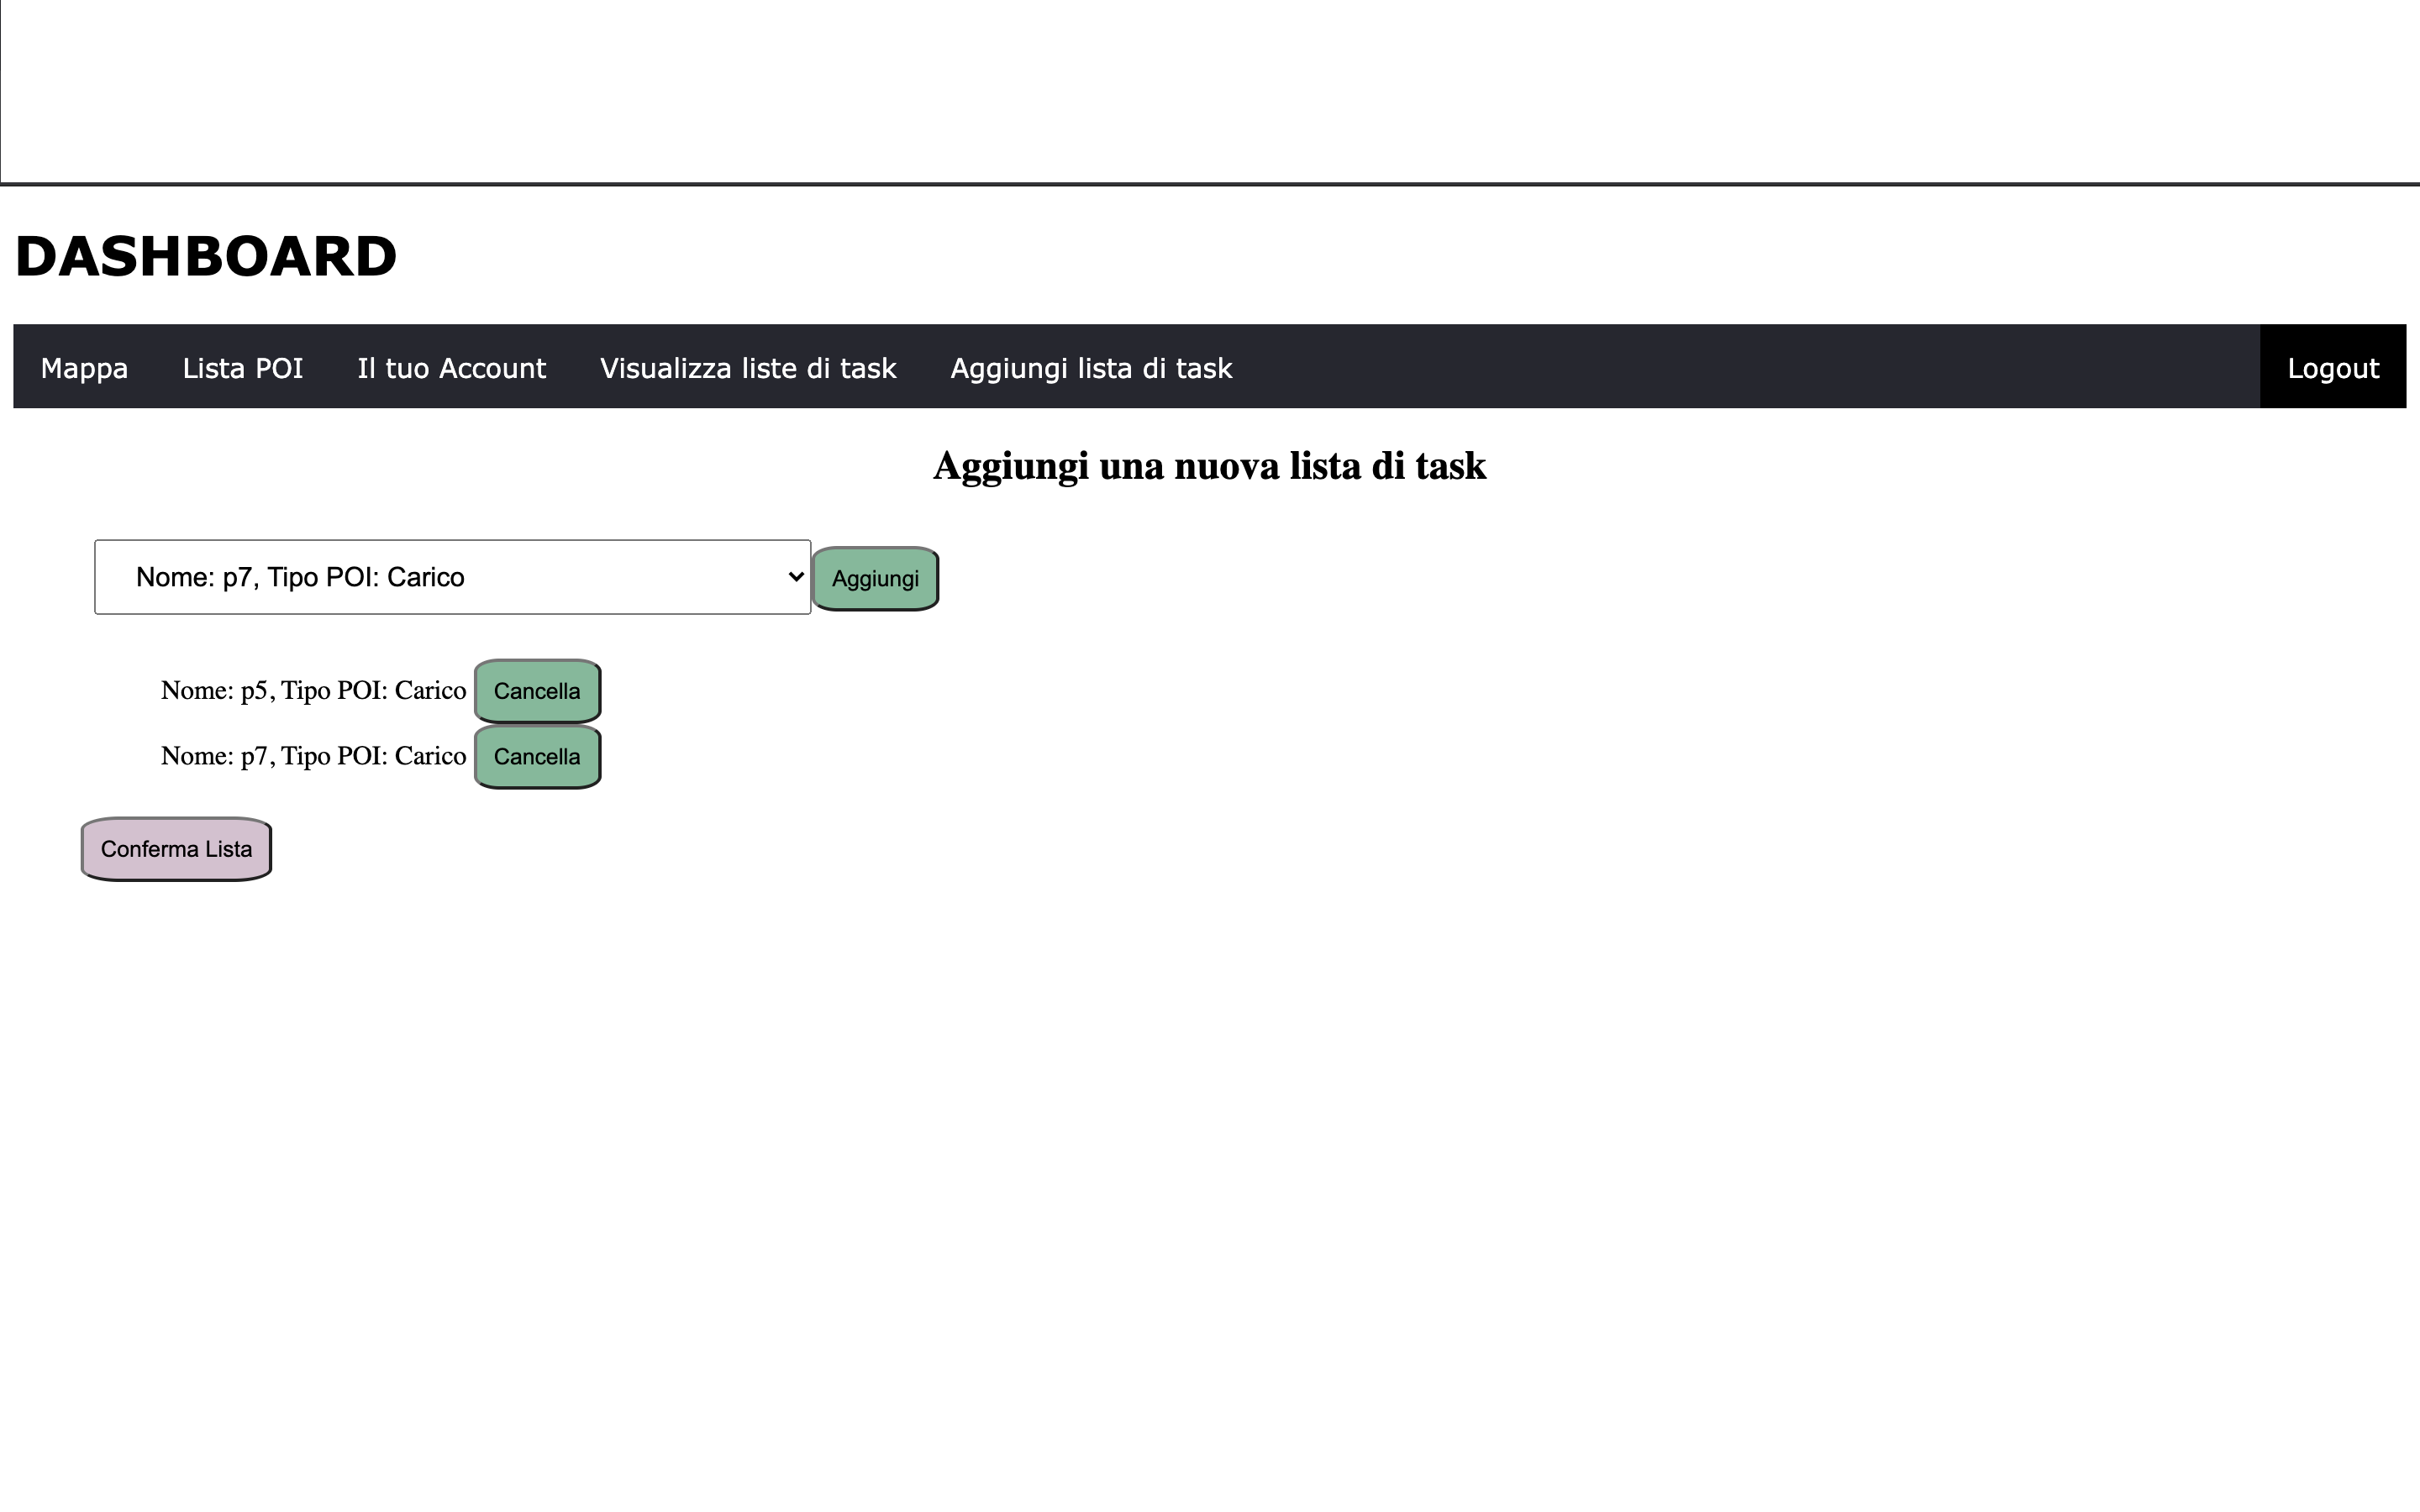
\includegraphics[scale=0.12]{res/images/newtask_manager.png}
    \caption{Schermata guida automatica dell'unità}
\end{figure}

\subsubsection{Eliminare una lista di task non ancora assegnata}
\begin{itemize}
    \item Premere sul pulsante "Elimina lista di task"
    \item viene visualizzata la lista di task non ancora assegnate;
    \item tramite il pulsante "Elimina" di fianco ad ogni lista è possibile eliminare la lista;
    \item per tornare alla pagina iniziale serve premere sul pulsante "Chiudi".
\end{itemize}
\begin{figure}[H]
    \centering
    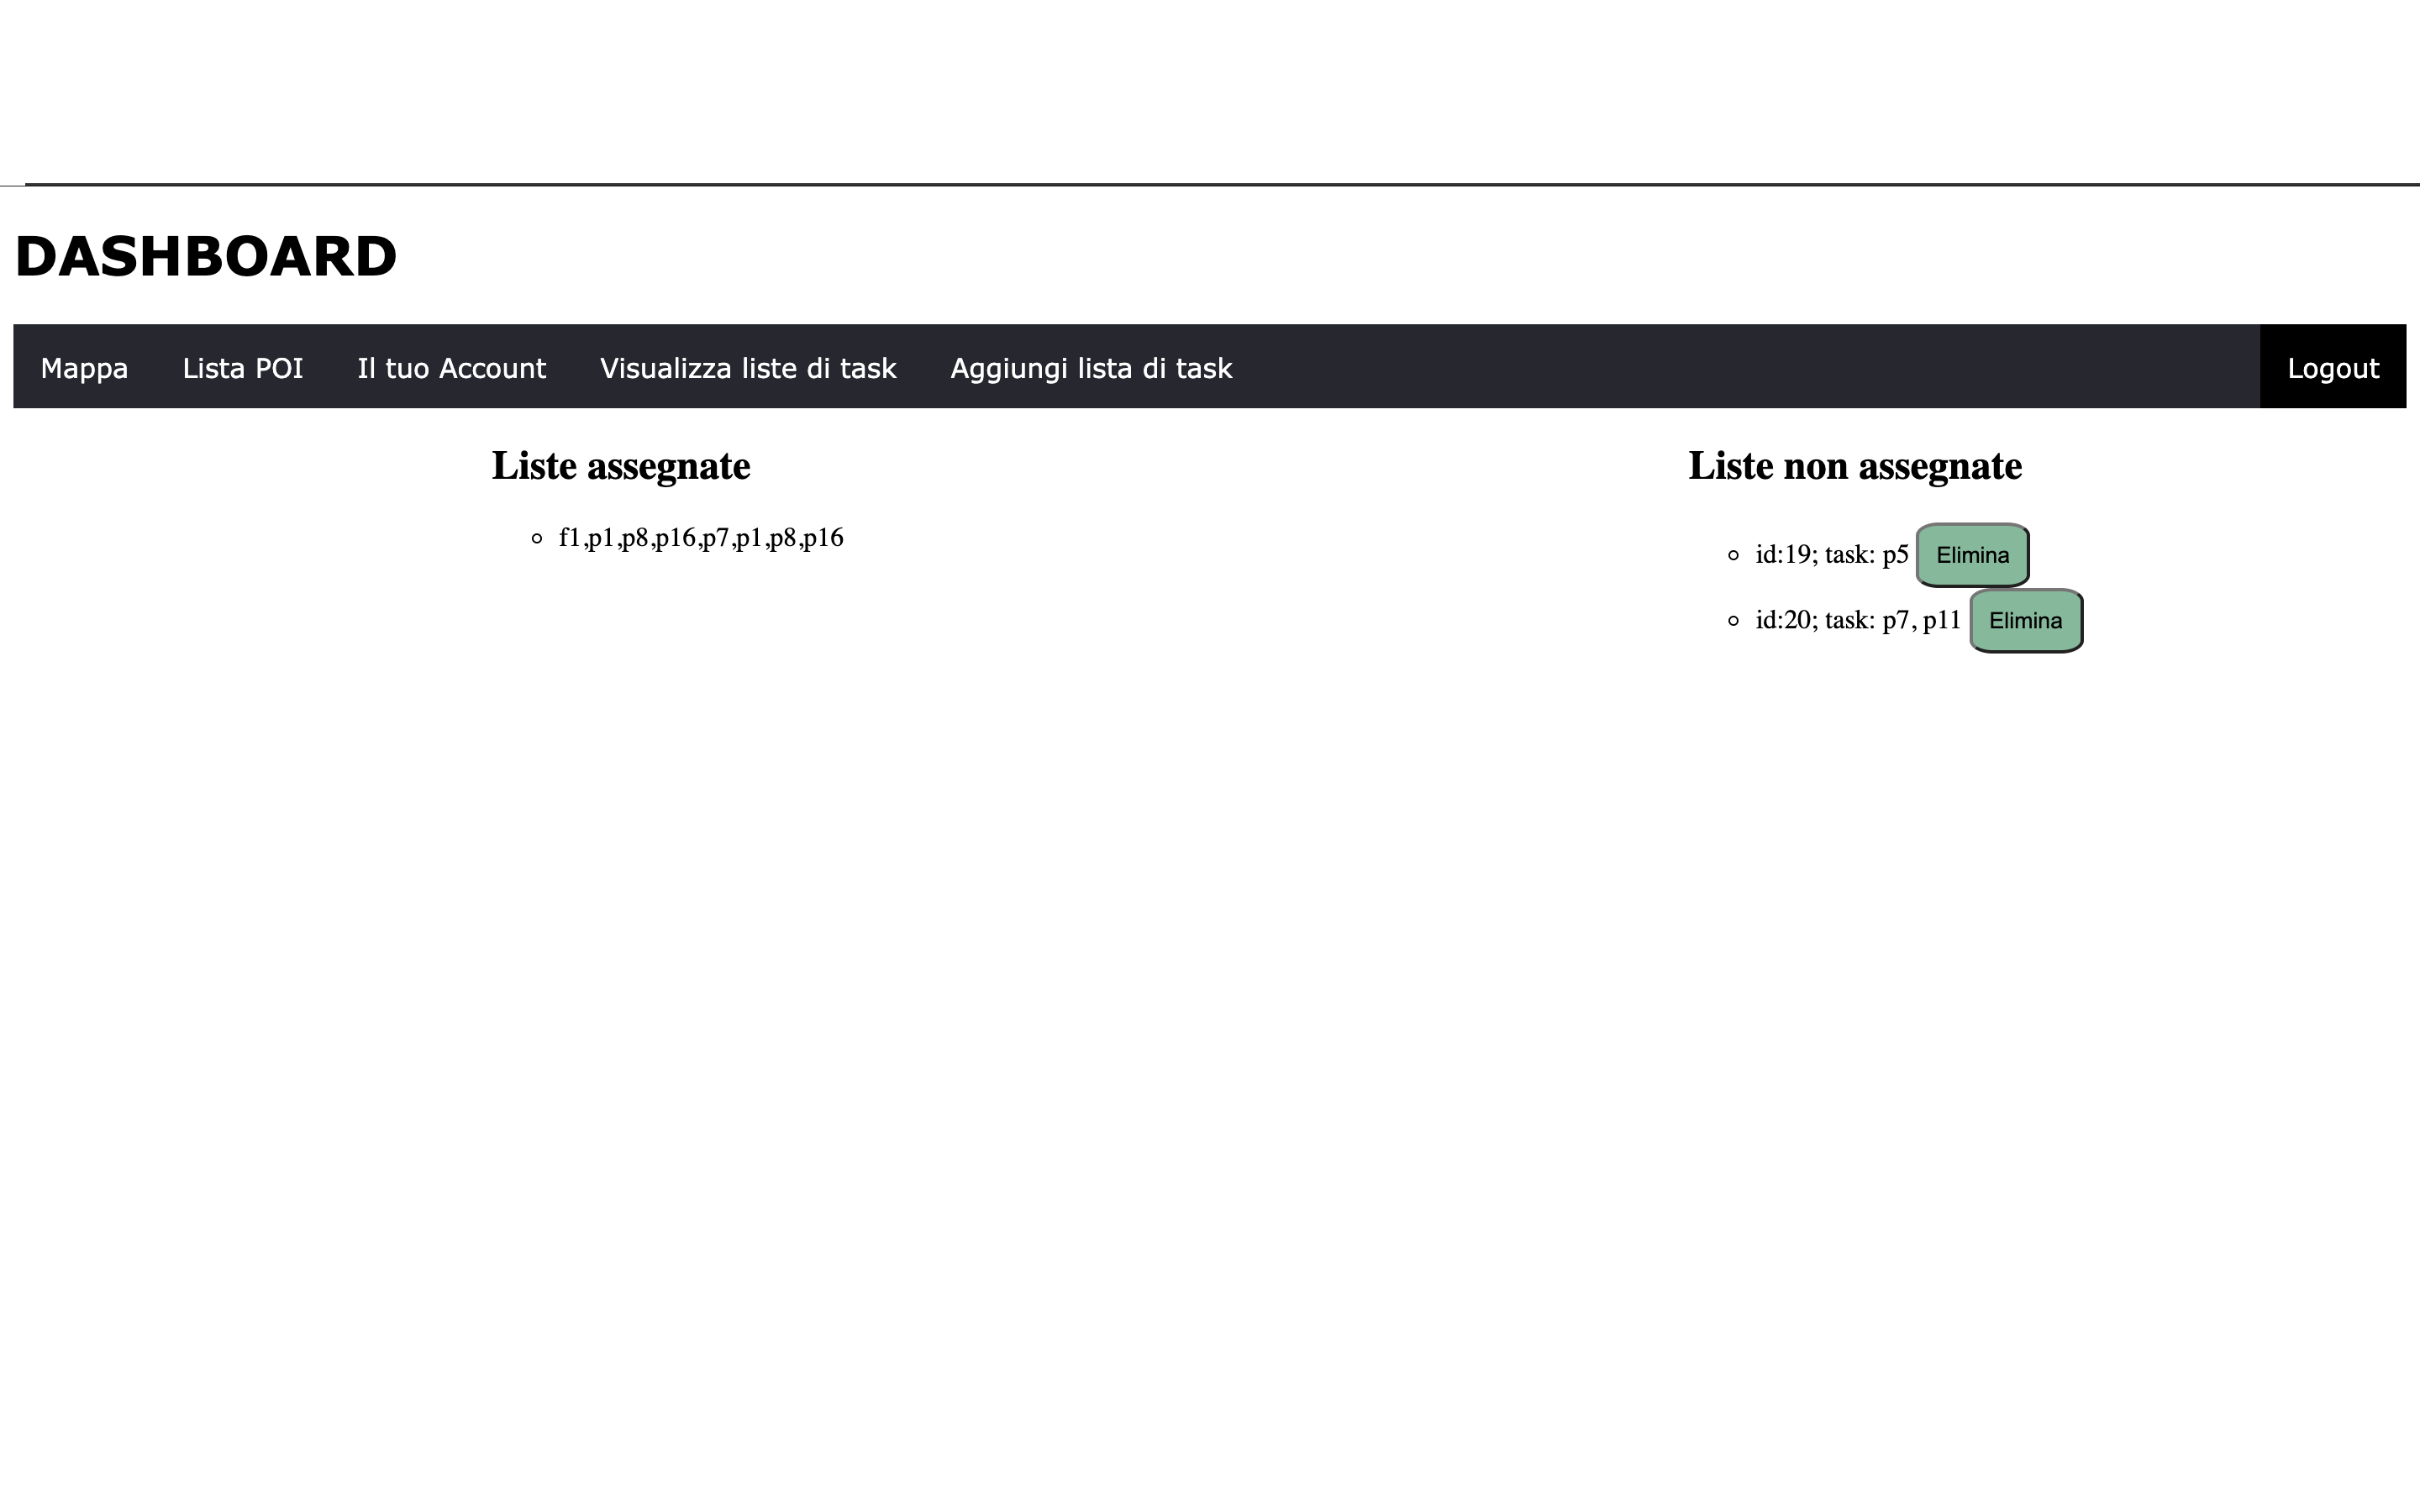
\includegraphics[scale=0.12]{res/images/task_manager.png}
    \caption{Schermata guida automatica dell'unità}
\end{figure}